\begin{figure*}[t]
\centering
\begin{tabular}{cccc}
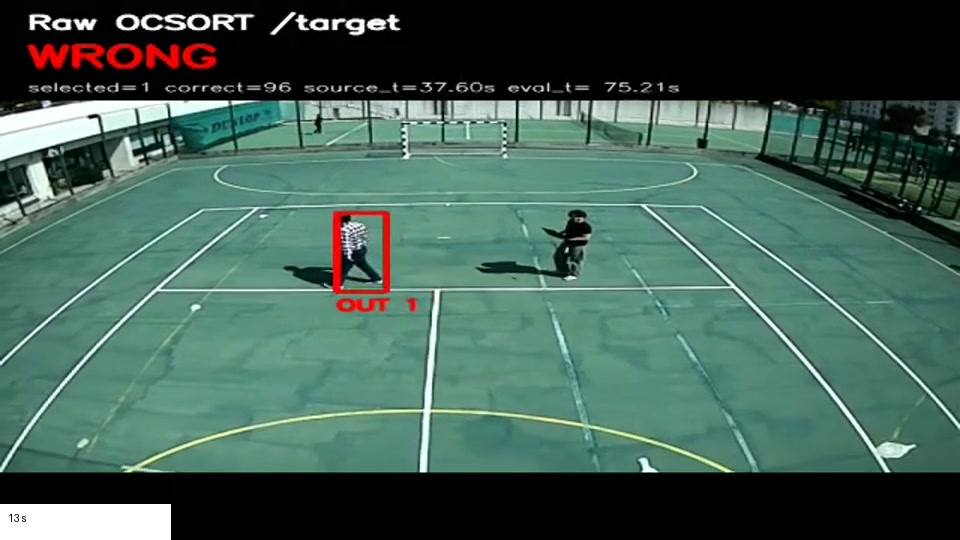
\includegraphics[width=0.235\textwidth]{figures/qual_raw_wrong_crop.jpg} &
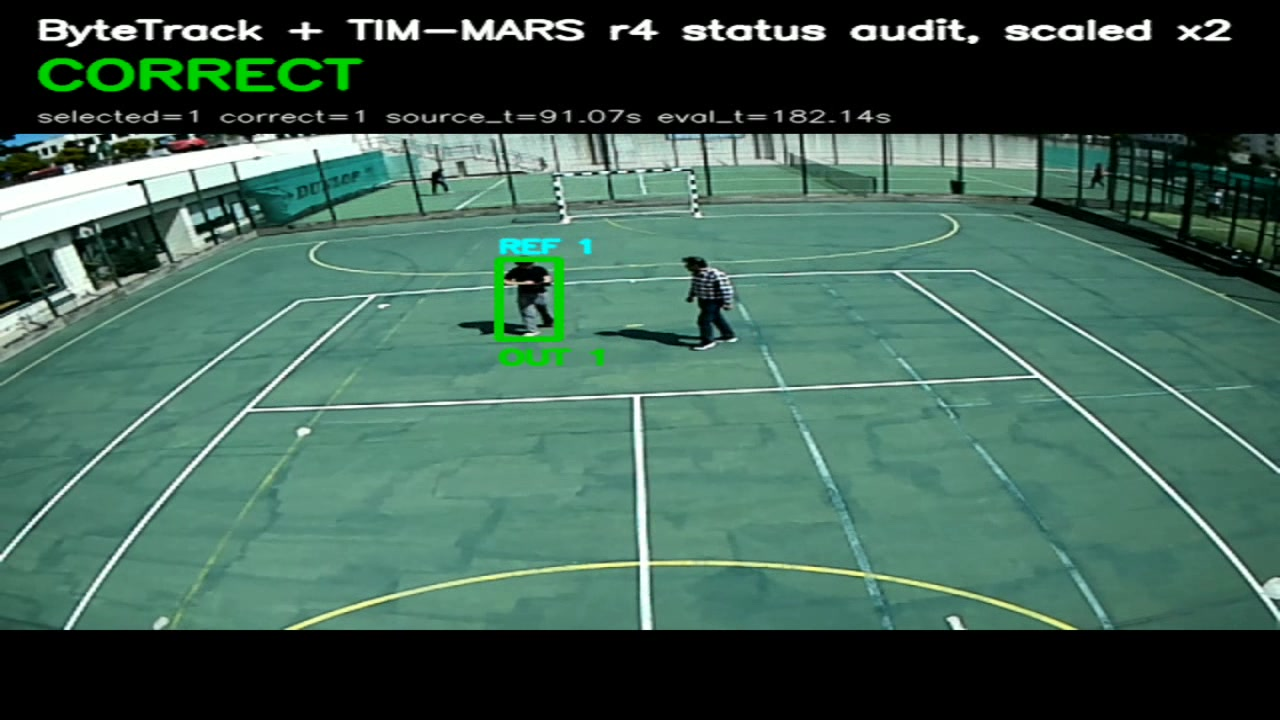
\includegraphics[width=0.235\textwidth]{figures/qual_tim_safe.jpg} &
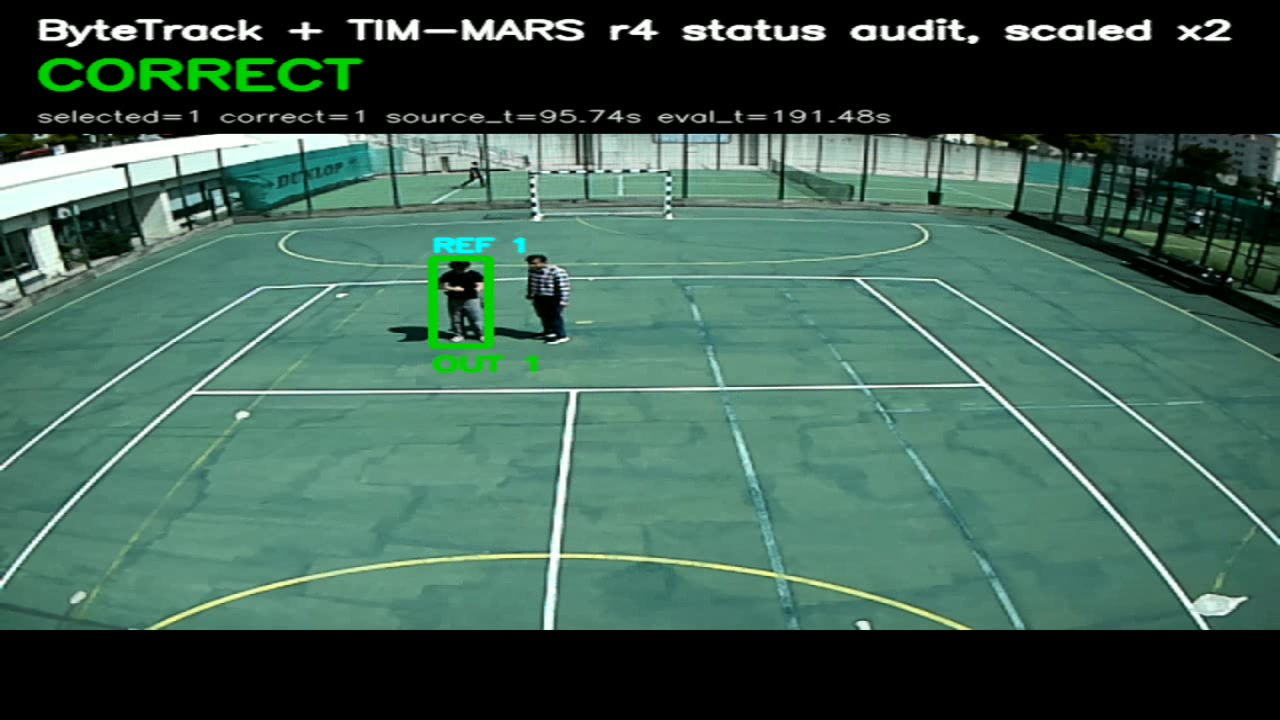
\includegraphics[width=0.235\textwidth]{figures/qual_reentry.jpg} &
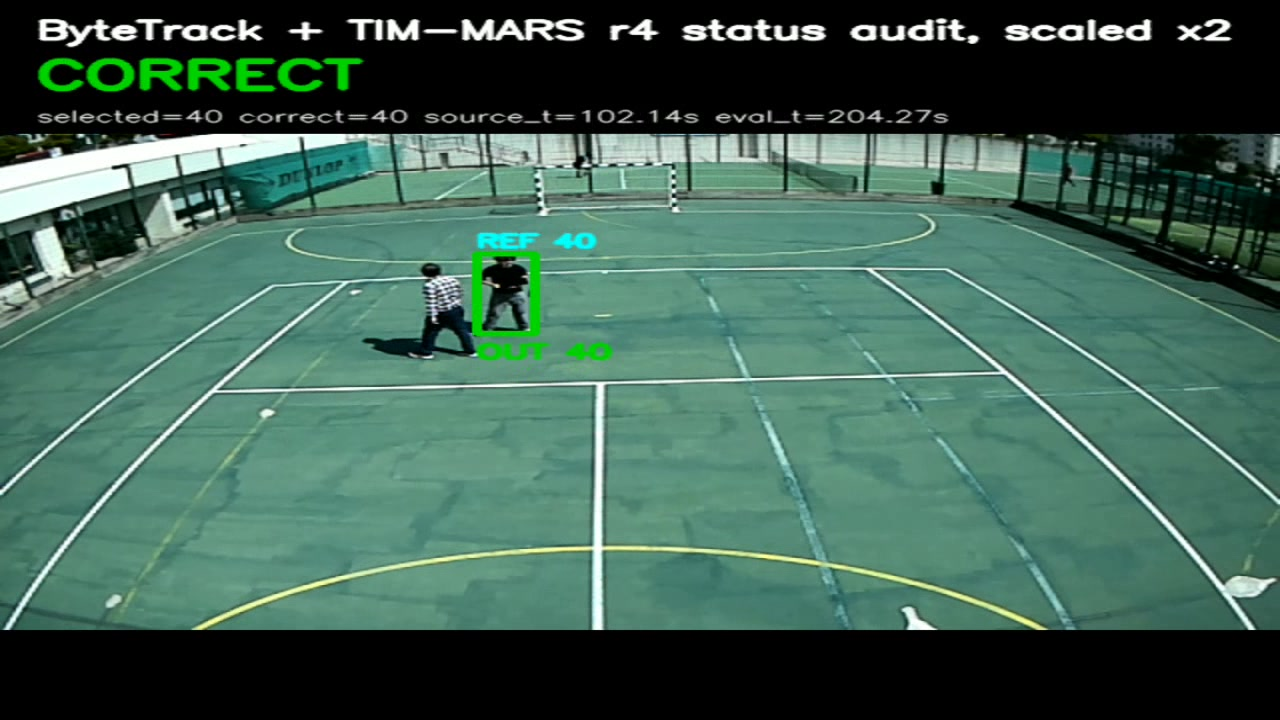
\includegraphics[width=0.235\textwidth]{figures/qual_reacquired.jpg} \\
(a) Raw OCSORT error &
(b) TIM-MARS correct selection &
(c) Close re-entry ambiguity &
(d) Correct identity recovery
\end{tabular}
\caption{Qualitative examples from the hard re-entry sequence. Panel (a) shows a representative raw selected-target failure, where the output persists on the wrong person. Panels (b)--(d) show ByteTrack + TIM-MARS maintaining and recovering the intended target identity after close interaction, even when the numeric tracker ID changes.}
\label{fig:qualitative_hard_reentry}
\end{figure*}
